\documentclass[a4paper,12pt]{article}

% Set margins
\usepackage[hmargin=2.5cm, vmargin=3cm]{geometry}

\frenchspacing

% Language packages
\usepackage[utf8]{inputenc}
\usepackage[T1]{fontenc}
\usepackage[magyar]{babel}

% AMS
\usepackage{amssymb,amsmath}

% Graphic packages
\usepackage{graphicx}

% Colors
\usepackage{color}
\usepackage[usenames,dvipsnames]{xcolor}
\usepackage{plantuml}

% Enumeration
\usepackage{enumitem}

% Links
\usepackage{hyperref}

\begin{document}

\begin{center}
	{\Large \textbf{Szakdolgozat bírálati folyamat és Záróvizsga menedzselő webalkalmazás - Specifikáció}}

	\bigskip
	
	{\large Drig Dávid}
\end{center}

\tableofcontents

\section{Bevezetés}

A dokumentum az elkészítendő webalkalmazás specifikációját tartalmazza.

\section{Szerepkörök}

A következő szakaszok a rendszer szereplőit, az általuk elérhető funkciókat, a szakdolgozat bírálati folyamat és a Záróvizsga során elvégzendő feladataikat tartalmazzák.

\subsection{Hallgató}

A hallgató, aki be szeretné nyújtani a szakdolgozatát, meg szeretné védeni, és záróvizsgázni szeretne.

\begin{itemize}
\item Szakdolgozat létrehozása, szerkesztése és mentése a rendszerben.
\item Az elkészült dolgozat benyújtása a rendszeren keresztül.
\item Visszajelzések és észrevételek megtekintése a dolgozatról a bírálók, témavezető vagy a bizottság részéről.
\item A bírálók és a bizottság értékeléseinek megtekintése.
\item A védés időpontjának és helyszínének megtekintése és kezelése.
\item A végső értékelés és jegy megtekintése.
\end{itemize}

\subsection{Bíráló}

A szakdolgozat szakmai elbírálására felkért külső bíráló.

\begin{itemize}
	\item A dolgozat értékelése és visszajelzés küldése a hallgatónak.
	\item A dolgozat nyomon követése és annak státuszának frissítése a rendszerben.
	\item Az értékelőlap és a végső jegy rögzítése a rendszerben.
\end{itemize}

\subsection{Jegyző}

A Záróvizsga jegyzője.

\begin{itemize}
	\item A záróvizsga időpontjának és helyszínének meghatározása és frissítése.
	\item A záróvizsga résztvevőinek (hallgató, bírálók, bizottság) értesítése és meghívók kiküldése.
	\item A záróvizsga jegyzőkönyvének vezetése és rögzítése a rendszerben.
\end{itemize}

\subsection{Elnök}

Záróvizsga bizottság elnöke:

\begin{itemize}
	\item A bizottság tagjainak kijelölése és módosítása.
	\item A záróvizsga menetének és a kérdéseknek meghatározása.
	\item A hallgató szakdolgozatának értékelése a bizottság véleménye alapján.
	\item A végső értékelés rögzítése a rendszerben.
\end{itemize}

\subsection{Témavezető}

A szakdolgozat témavezetője. (A konzulens a rendszerben csak névlegesen szerepel. Nem külön szerepkör.)

\begin{itemize}
	\item A hallgatóval való kommunikáció és támogatás a szakdolgozat elkészítése során.
	\item A hallgató dolgozatának nyomon követése és visszajelzések küldése.
	\item A bírálók és a bizottság értékeléseinek megtekintése.
	\item A végső értékelés és jegy rögzítése a rendszerben.
\end{itemize}

\section{Bírálati folyamat}

A következő szakaszokban a bírálati folyamat részletezését láthatjuk különféle szempontokból, szerepkörökből.

\subsection{Optimista eset}

A rendszer célja, hogy hatékonyan kezelje a szakdolgozatok Bírálati Folyamatát és a kapcsolódó érintett szereplők közötti kommunikációt. A leírás az alábbi lépéseket foglalja össze:

\begin{enumerate}
\item Elnök felkéri a Hallgatót a regisztrációra: A folyamatot az Elnök indítja, amikor felkéri a Hallgatót, hogy regisztráljon a rendszerbe. Ez a lépés azt jelenti, hogy a Hallgatónak lehetősége van hozzáférni a szakdolgozat bírálati folyamatához.

\item Hallgató sikeresen regisztrál: A Hallgató sikeresen regisztrál a rendszerbe, és így jogosultá válik a szakdolgozatának bírálati folyamatára.

\item Elnök felkéri a Témavezetőt a bírálatra: Az Elnök felkéri a Témavezetőt, hogy végezze el a szakdolgozat bírálatát. Ez a lépés azt jelzi, hogy a Témavezetőnek feladata van értékelni és észrevételeket tenni a szakdolgozatról.

\item Témavezető felkéri a Bírálót a bírálatra: A Témavezető felkéri a Bírálót, hogy részt vegyen a szakdolgozat bírálatában. A Bíráló feladata a szakdolgozat objektív értékelése és véleményezése.

\item Bíráló elküldi a bírálatot az Elnöknek: A Bíráló elkészíti a bírálatát a szakdolgozatról, és elküldi azt az Elnöknek. Ez a lépés azt jelenti, hogy a Bíráló megosztja az észrevételeit és értékelését a szakdolgozatról a rendszer adminisztrátorával.

\item Témavezető elküldi a bírálatot az Elnöknek: A Témavezető szintén elkészíti a saját bírálatát a szakdolgozatról, és azt az Elnöknek küldi el. Ez a lépés lehetővé teszi, hogy mind a Témavezető, mind a Bíráló észrevételeit összevetve az Elnök döntést hozzon a szakdolgozattal kapcsolatban.
\end{enumerate}

\subsection{Többszörös bírálói felkérés}

Ez a szekvenciadiagram lépésről lépésre bemutatja a Többszörös Bírálói Felkérés Folyamatát, a felkéréstől a végleges bírálati visszajelzésig. A leírás az alábbi lépéseket foglalja össze:

\begin{enumerate}
\item Felkérés a regisztrációra: A folyamatot az Elnök indítja, amikor felkéri a Hallgatót, hogy regisztráljon a rendszerbe. Ez a lépés azt jelenti, hogy a Hallgatónak lehetősége van hozzáférni a szakdolgozat bírálati folyamatához.

\item Hallgató sikeresen regisztrál: A Hallgató sikeresen regisztrál a rendszerbe, és így jogosultá válik a szakdolgozatának bírálati folyamatára.

\item Elnök felkéri a Témavezetőt a bírálatra: Az Elnök felkéri a Témavezetőt, hogy végezze el a szakdolgozat bírálatát. Ez a lépés azt jelzi, hogy a Témavezetőnek feladata van értékelni és észrevételeket tenni a szakdolgozatról.

\item Témavezető felkéri a Bírálót a bírálatra: A Témavezető felkéri a Bírálót, hogy részt vegyen a szakdolgozat bírálatában. A Bíráló feladata a szakdolgozat objektív értékelése és véleményezése.

\item Elfogadás: A Bíráló elfogadja a felkérést, és ezt jelzi.

\item Visszautasítás: A Bíráló visszautasítja a felkérést, és ezt jelzi.

\item Visszajelzés a bírálókról: A Témavezető visszajelzést ad az Elnöknek a bírálók elfogadásáról vagy visszautasításáról.

\item Bíráló elküldi a bírálatot az Elnöknek: A Bíráló elkészíti a bírálatát a szakdolgozatról, és elküldi azt az Elnöknek. Ez a lépés azt jelenti, hogy a Bíráló megosztja az észrevételeit és értékelését a szakdolgozatról a rendszer adminisztrátorával.

\item Témavezető elküldi a bírálatot az Elnöknek: A Témavezető szintén elkészíti a saját bírálatát a szakdolgozatról, és azt az Elnöknek küldi el. Ez a lépés lehetővé teszi, hogy mind a Témavezető, mind a Bíráló észrevételeit összevetve az Elnök döntést hozzon a szakdolgozattal kapcsolatban.
\end{enumerate}

\subsection{Hallgatók felvitele}

Ez a szekvenciadiagram részletesen szemlélteti a Hallgatók felvitele folyamatát az adatok megadásától az adatlap jóváhagyásának értesítéséig, mindezt az Elnök, Hallgató és Jegyző közötti interakciókkal.

\begin{enumerate}
\item Hallgató adatok megadása: Az Elnök megadja a Hallgató adatait a rendszerben, hogy felkészüljenek a regisztrációra. Az adatok tartalmazzák a szükséges információkat a Hallgatóról.

\item Adatok ellenőrzése és validáció: Az Elnök ellenőrzi és érvényesíti az adatokat, hogy biztos legyen a hitelességükben és a pontosságukban.

\item Felvételre kerülés értesítése: Az Elnök értesíti a Hallgatót a sikeres felvételről, és arról, hogy részt vehet a folyamatban.

\item Belépés a rendszerbe: A Hallgató belép a rendszerbe a saját fiókjába, hogy folytassa a felvételi folyamatot.

\item Adatlap kitöltése: A Hallgató kitölti az adatlapját a szükséges információkkal.

\item Új adatlap értesítése: A Hallgató elküldi az újonnan kitöltött adatlapot a Jegyzőnek, jelezve a további folyamat kezdetét.

\item Adatlap ellenőrzése: A Jegyző értesül arról, hogy új adatlap érkezett, majd alaposan ellenőrzi az adatokat és a kitöltött információkat.

\item Visszajelzés és jóváhagyás: A Jegyző visszajelzést küld a Hallgatónak az adatlap jóváhagyásáról, és esetleges korrekciókról, ha szükséges.

\item Adatlap jóváhagyása: Miután az adatlapot jóváhagyásra alkalmasnak találták, a Jegyző hivatalosan is jóváhagyja az adatlapot.

\item Értesítés a jóváhagyásról: A Jegyző értesíti az Elnököt az adatlap jóváhagyásáról és a felvétel sikerességéről.

\item Adatlap jóváhagyásának értesítése a Hallgatónak: Az Elnök értesíti a Hallgatót az adatlap jóváhagyásáról és a felvétel megerősítéséről.
\end{enumerate}

\subsection{Témavezető bírálati folyamat}

A folyamatábra bemutatja a szakdolgozat bírálat feltöltésének folyamatát a Témavezető és a Bíráló között (\ref{fig:Biralat_Feltoltes}. ábra).

\begin{figure}
\centering
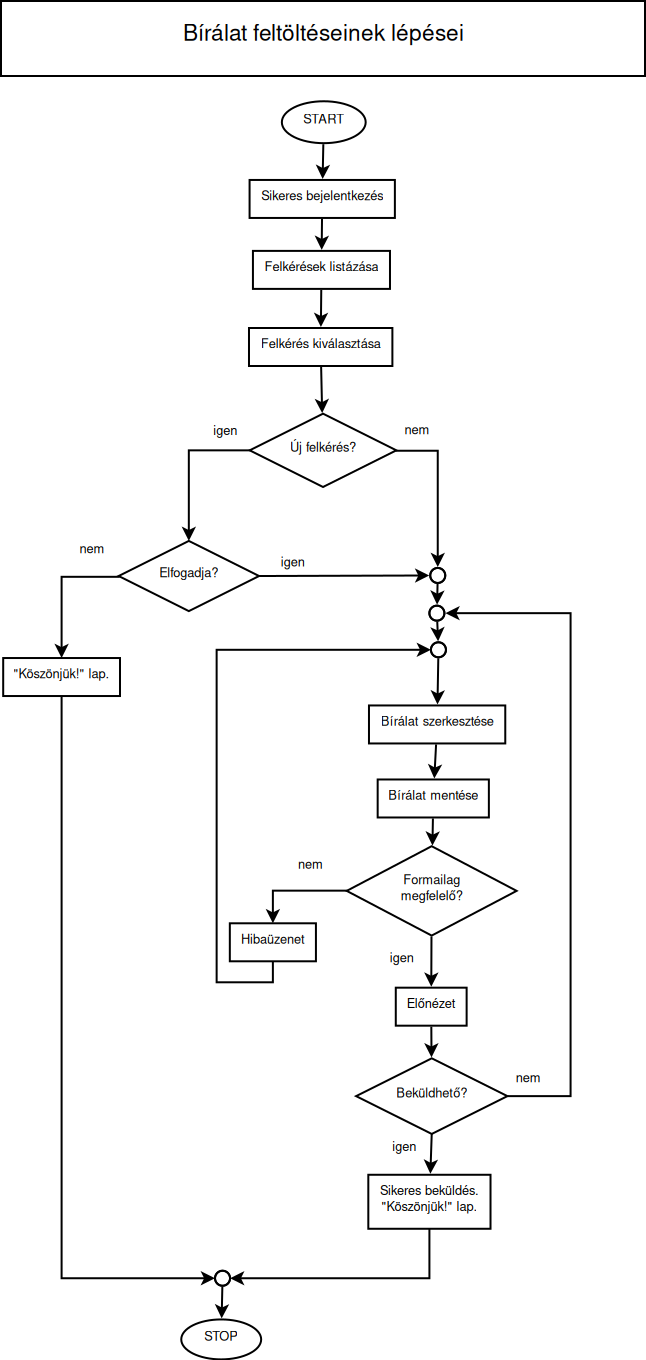
\includegraphics[scale=0.45]{images/Folyamatabra/Biralat_Feltoltes.png}
\caption{Bírálat feltöltés folyamata}
\label{fig:Biralat_Feltoltes}
\end{figure}

\begin{enumerate}
\item A Témavezető és a Bíráló bejelentkezik: A Témavezető és a Bíráló is bejelentkezik a rendszerbe, hogy hozzáférjenek a szükséges funkciókhoz.

\item Témavezető kilistázza és kiválasztja a Bírálót: A Témavezető megjeleníti a rendszerben elérhető Bírálók listáját és a Témavezető kiválasztja a Bírálót.

\item Felhasználók kiválasztják a szakdolgozatot: Mind a Témavezető, mind a Bíráló kiválasztja a szakdolgozatot, amelyre a bírálatot el szeretné készíteni.

\item A Felhasználók megírják a bírálatot: Mind a Témavezető, mind a Bíráló megírja a bírálatot.

\item Bírálat mentése és feldolgozása a rendszerben: A rendszer elmenti és feldolgozza a feltöltött bírálatot.

\item Rendszer ellenőrzi, hogy a bírálat PDF formátumban van és érvényes-e: A rendszer ellenőrzi, hogy a bírálat valóban PDF formátumban van-e és érvényes-e.

\item Rendszer előnézetet készít a bírálatból: A rendszer előnézetet készít a bírálatból, hogy a Témavezető és a Bíráló ellenőrizhesse a dokumentumot.

\item Témavezető szerkeszti a bírálatot (szükség esetén): A Témavezető lehetősége van szerkeszteni a bírálatot, ha szükségesnek látja.

\item Bíráló szerkeszti a bírálatot (szükség esetén): A Bírálónak is lehetősége van szerkeszteni a bírálatot, ha szükségesnek tartja.

\item Bírálat véglegesítése és mentése a rendszerben: A Témavezető és a Bíráló véglegesíti a szerkesztéseket, majd a rendszer elmenti a végleges bírálatot.

\item Visszajelzés a rendszerben a Témavezetőnek és a Bírálónak: A rendszer visszajelzést küld mind a Témavezetőnek, mind a Bírálónak arról, hogy a bírálatuk sikeresen rögzítésre került.

\item Témavezető és a Bíráló megtekinti a bírálatot: Végül mind a Témavezető, mind a Bíráló megtekinti a véglegesített bírálatot a rendszerben.
\end{enumerate}

\begin{plantuml}
	@startuml
	Alice -> Bob: Hello
	Alice <- Bob: Hi!
	@enduml
\end{plantuml}

\section{Összegzés}

\end{document}
